% !TEX root = ./Vorlesungsmitschrift DIFF 2.teX
\chapter{Metrische Räume}
\lecture{Mo 20.04. 10:15}{}
\begin{ziel*}
    Konvergenz, Stetigkeit \ldots sollten in einem allgemeineren Rahmen konzeptualisiert werden.
\end{ziel*}
\begin{erinnerung*}[\diffcourse{1}]
    Eine Folge \( (a_n)_{n\in \naturals}\subset \reals \) konvergiert gegen den Grenzwert \( a \)
    \begin{align*}
        \iff \forall \varepsilon>0 \logicspace\exists N\in \naturals\logicspace\text{\sd}\logicspace \abs{a_n-a}<\varepsilon\logicspace\forall n \geq N
    \end{align*}
    \( \ointerval{a-\varepsilon}{a+\varepsilon} \) wird auch \( \varepsilon \)-Umgebung von \( a \) in \( \reals \) genannt. 
    Somit lautet die obige Definition in Worten: 
    In jeder noch so kleinen \( \varepsilon \)-Umgebung von a befinden sich alle bis auf endlich viele Folgenglieder.    
\end{erinnerung*}
Man benötigt für die Formulierung der Definition also lediglich einen Begriff von \enquote{(kleine) Umgebung}. 
Diesen Begriff möchten wir nun verallgemeinern.
    
\begin{definition}\label{topologie}\index{Topologie}
    Sei \( X \) eine Menge. Ein System \( \mathcal{T} \) von Teilmengen von \( X \) heißt Topologie auf \( X \) falls gilt: 
    \begin{eigenschaftenenumerate}
        
        \item\label{topologie:grundmengen} \( \emptyset,X\in \mathcal{T} \).
        \item\label{topologie:endlicher_schnitt} Sind \( U \) und \( V\in \mathcal{T} \), so gilt \( U\cap V \in \mathcal{T}\).
        \item\label{topologie:unendliche_vereinigung} Ist \( I \) eine Indexmenge und \( U_i \in \mathcal{T}  \) für alle \( i\in I \), so gilt auch \( \bigcup_{i\in I}U_i\in \mathcal{T} \).
    \end{eigenschaftenenumerate}
    
\end{definition}
\begin{notation*}
    Ein topologischer Raum ist ein Tupel \( (X,\mathcal{T}) \), wobei \(X\) Menge ist und \( \mathcal{T} \) eine Topologie auf \(X\).

    Eine Teilmenge \( U \subset X \) heißt \emph{offen}, falls gilt \(U \in \mathcal{T}\).
    Eine Teilmenge \(A \subset X\) heißt \emph{abgeschlossen} falls ihr Komplement \(X \setminus A\) offen ist.
        
    
\end{notation*}
\begin{beispiele}
    \begin{enumerate}
        \item \label{klumpentopologie}\( X= \) beliebige Menge. \( \mathcal{T}=\Set{\emptyset, X} \).
        \begin{proof}
            \begin{proofdescription}
                
                \item[\ref{topologie:grundmengen}] klar
                \item[\ref{topologie:endlicher_schnitt}] \( \emptyset\cap X=\emptyset\in \mathcal{T} \), \( X\cap X=X\in \mathcal{T} \), \( \emptyset\cap \emptyset=\emptyset\in \mathcal{T} \)
                \item[\ref{topologie:unendliche_vereinigung}] \( \bigcup_{i\in I}U_i=\begin{cases}
                    X & \text{falls eins der \( U_i=X \) ist}\\
                    \emptyset & \text{falls nicht}
                \end{cases}
                    \) 
            \end{proofdescription}               
        \end{proof}
        \enquote{Klumpentopologie}
        
        \item \label{standard-topologie}\( X=\reals \)\\
        \( \mathcal{T}= \) alle Teilmengen \( U\subset \reals \) mit der Eigenschaft:
        \begin{align*}
            \forall  x\in U\logicspace\exists\varepsilon>0\logicspace\text{\sd}\logicspace \ointerval{x-\varepsilon}{x+\varepsilon}\subset U
        \end{align*}
        Beweis von \ref{topologie:grundmengen}, \ref{topologie:endlicher_schnitt} und \ref{topologie:unendliche_vereinigung} als HA (etwas allgemeiner).
        Hier stellen wir fest, dass insbesondere die offenen Intervalle \( \ointerval{a}{b} \) in diesem Sinne offen (also \( \in \mathcal{T} \)) sind, halb-abgeschlossene und abgeschlossene dagegen nicht.
        \begin{proof}
            \begin{proofenumerate}[label=\textbf{\arabic*. Beh}]
                \item Zu \( x\in \interval{a}{b} \) wähle \( \varepsilon=\Min{\Set{\abs{x-a},\abs{x-b}}} \)
                \item Zu \( x=a\in \rinterval{a}{b} \) kann man kein \( \varepsilon>0 \) finden \sd \( \ointerval{a-\varepsilon}{a+\varepsilon}\subset \rinterval{a}{b} \),
                denn \( a-\varepsilon/2\in \ointerval{a-\varepsilon}{a+\varepsilon} \) aber \( a-\varepsilon/2<a \), also \( \notin \rinterval{a}{b} \).
            \end{proofenumerate}
            
            
        \end{proof}
        Abgeschlossene Intervalle sind in diesem Sinn abgeschlossen, denn \( \reals\setminus \interval{a}{b} \) ist nach Definition von \( \mathcal{T} \) und Eigenschaft \ref{topologie:unendliche_vereinigung} offen.

        Diese Topologie heißt Standard-Topologie auf \( \reals \). 
        Wird nichts anderes gesagt, sehen wir \(\reals \) als mit der Standard-Topologie versehen an.
    \end{enumerate}
\end{beispiele}
\begin{definition}\label{umgebung_in_topologischen_raeumen}\index{Umgebung}
    Sei \( (X, \mathcal{T}) \) topologischer Raum. 
    Sei \( x\in X \). 
    Eine Teilmenge \( V\subset X \) heißt \emph{Umgebung von \( x \)}, falls es eine offenen Menge \( U\subset X \) gibt mit \( x\in U \) und \( U\subset V \).
\end{definition}
\begin{beispiele*}
    \begin{enumerate}
        \item \( V=\ointerval{a}{b} \) ist eine Umgebung für jedes \( x\in \ointerval{a}{b} \), aber \emph{nicht} für \( x=a \).
        \begin{figure}[H]
            \centering
            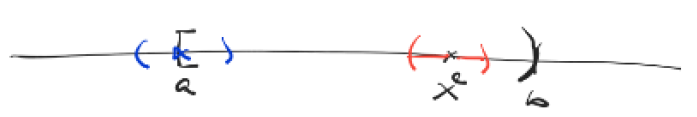
\includegraphics[width=0.7\linewidth]{figures/umgebung_beispiel_halboffenes_intervall}
            \label{fig:umgebung_beispiel_halboffenes_intervall}
        \end{figure}
        
        \item \( \ointerval{a-\varepsilon}{a+\varepsilon} \),  \( \varepsilon>0 \), ist eine Umgebung von \( a \).         
    \end{enumerate}
\end{beispiele*}
\begin{lemma}\label{offene_menge_umgebung_aller_elemente}
    Eine Teilmenge \( V\subset X \) eines topologischen Raumes \( (X,\mathcal{T}) \) ist offen \gdw für alle \( x\in V \) gilt: \( V \) ist Umgebung von \( x \).
\end{lemma}
\begin{proof}
    \begin{proofdescription}
        
        \item[\hin] Ist \( V \) offen, so erfüllt \( U=V \) für jedes \( x \) die Bedingung \( x\in U \) und \( U\subset V \) \timplies \( V \) ist Umgebung.
        \item[\rueck] Zu \( x\in V \) wähle \( U_x \) \sd \( x\in U_x \), \( U\subset V \). 
        Dann gilt \( V=\bigcup_{x\in U} U_x \) und das ist offen (nach \ref{topologie:unendliche_vereinigung}).
    \end{proofdescription}
    
    
\end{proof}
\begin{definition}[Konvergenz in topologischen Räumen] \label{konvergenz_in_topologischen_raeumen}\index{Konvergenz}
    Sei \( (X, \mathcal{T}) \) topologischer Raum.
    Sei \( (x_n)_{n\in \naturals} \) eine Folge in \( X \).
    Dann ist \( (x_n)_{n} \) \emph{konvergent mit Grenzwert \( x \)}, \( x_n\goesto x \) in \( (X, \mathcal{T}) \), falls es in jeder Umgebung \( V \) von \( x  \) ein \( N\in \naturals \) gibt, \sd \( x_n\in V\logicspace\forall n\geq N \).
    
\end{definition}

\begin{beispiele*}
    \begin{enumerate}
        \item In der Klumpentopologie konvergieren alle Folgen gegen jedes \( x\in X \).
        \item Mit unseren obigen Überlegungen folgern wir, dass Konvergenz in \( \reals \) im Sinn von \thref{konvergenz_in_topologischen_raeumen} mit Konvergenz, wie wir sie in der \diffcourse{1} kennengelernt haben.
    \end{enumerate}
\end{beispiele*}
\begin{lemma}\label{hausdorff_alle_grenzwerte_eindeutig}
    Sei \( (X,\mathcal{T}) \) topologischer Raum. 
    Ist \( (X, \mathcal{T}) \) ein \emph{Hausdorff-Raum}, gibt es also zu je zwei Punkten \( x,y\in X \) mit \( x\neq y \) Umgebungen \( U \) von \( x \) und \( V \) von \( y \) mit \( U \cap V=\emptyset \), so ist der Grenzwert einer konvergenten Folge eindeutig.
\end{lemma}
\begin{proof}
    Seien \( x \) und \( y \) Grenzwert einer Folge \( (x_n)_n \).
    Angenommen \( x\neq y \), so wähle \( U \) Umgebung von \( x \), \( V \) Umgebung von \( y \) mit \( U\cap V=\emptyset \). 
    Dann gibt es (wegen der Konvergenz) \( N \in \naturals \) \sd \( x_n \in U \logicspace\forall n \geq N \) und \( M\in \naturals \) \sd \( x_n \in V \logicspace \forall n \geq M \). 
    Widerspruch zu \( U\cap V = \emptyset \). 
\end{proof}
\begin{definition}\label{stetigkeit_in_topologischen_raeumen}\index{Stetigkeit}
    Seien \( (X, \mathcal{T}) \) und \( (Y,\tilde{\mathcal{T}}) \) topologische Räume. 
    Sei \( f\maps X\to Y \) eine Abbildung. 
    Dann heißt \( f \) \emph{stetig in \( a\in X \)}, falls es zu jeder Umgebung \( V \) von \( f(a)\in Y \) eine Umgebung \( U \) von \( a \) gibt, \sd \( f(U)\subset V \). 
    \( f \) heißt \emph{stetig} (auf \( X \)), falls \( f \) stetig in allen \( a\in X \) ist.
\end{definition}
\begin{bemerkung*}
    Wir werden später sehen, dass diese Definition für \( f\maps \reals\to\reals \) mit unserer Definition aus der \diffcourse{1} übereinstimmt (\( \varepsilon \)-\( \delta \)-Kriterium).
\end{bemerkung*}
\begin{figure}[H]
    \centering
    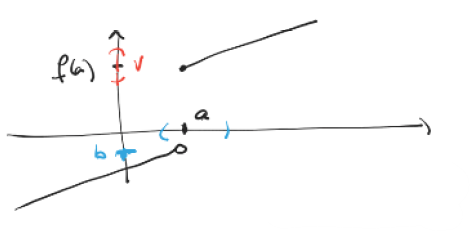
\includegraphics[width=0.6\linewidth]{figures/topologische_unstetigkeit_beispiel_aus_r}
    \caption*{\textcolor{Cyan}{Für jede Umgebung \( U \) von \( a \) gilt: \( f(U) \) enthält auch Punkte \( <b \), also außerhalb }\textcolor{OrangeRed}{\( V \)}}
    \label{fig:topologische_unstetigkeit_beispiel_aus_r}
\end{figure}
\begin{satz}\label{stetigkeit_in_topologischen_raeumen:urbildkriterium}
    Sei \( f\maps X\to Y \) Abbildung zwischen topologischen Räumen. 
    Dann ist \( f \) stetig auf \( X \) \gdw für jede offene Teilmenge \( V\subset Y \) das \emph{Urbild} \( \inverse{f}(V) \), also \( \Set{x\in X|f(x)\in V} \) offen in \( X \) ist.
\end{satz}
\begin{proof}
    \begin{proofdescription}
        
        \item[\hin] Sei \( f \) stetig vorausgesetzt.
        Sei \( V \) offen \( Y \). Ist das Urbild \( \inverse{f}(V) \) leer, sind wir fertig.
        
        Sei also \( a\in \inverse{f}(V) \). 
        Dann gibt es nach Voraussetzung eine Umgebung \( U \) von \( a \) \sd \( f(U)\subset V \). 
        Also gilt \( U \subset \inverse{f}(V)\). 
        Somit besitzt also jeder Punkt \( a\in \inverse{f}(V) \) eine Umgebung \( U \) mit \( U\subset \inverse{f}(V) \) und somit ist \( \inverse{f}(V) \) selbst Umgebung jedes seiner Elemente \( \overset{\ref{offene_menge_umgebung_aller_elemente}}{\implies} \inverse{f}(V)\) ist offen.

        
        \item[\rueck] Sei \( a\in X \) beliebig. Sei \( V \) eine Umgebung von \( f(a) \). Dann gibt es \( \tilde{V} \) offen mit \( f(a)\in \tilde{V} \) und \( \tilde{V}\subset V \). Nach Voraussetzung ist das Urbild \( U\definedas \inverse{f}(\tilde{V}) \) offen. \( U \) enthält \( a \), ist also Umgebung von \( a \) und es gilt \( f(U)=\tilde{V}\subset V \)\timplies \( f \) ist stetig in \( a \).
    \end{proofdescription}
    
\end{proof}
\begin{figure}[H]
    \centering
    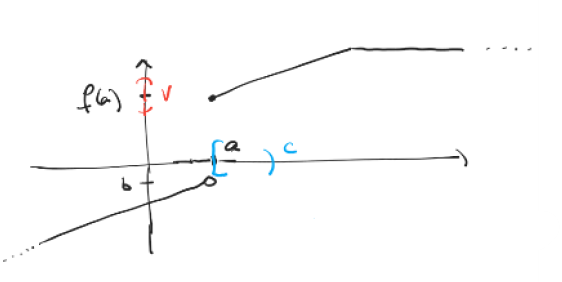
\includegraphics[width=0.8\linewidth]{figures/beispiel_urbild_offener_menge_unter_nicht_stetiger_abbildung_nicht_offen}
    \caption*{\textcolor{Cyan}{\( \inverse{f}(V)=\rinterval{a}{c} \) ist nicht offen in \( \reals \)}}
    \label{fig:beispiel_urbild_offener_menge_unter_nicht_stetiger_abbildung_nicht_offen}
\end{figure}
\begin{bemerkung*}
    Äquivalent: \( f \) ist genau dann stetig, wenn das Bild jeder abgeschlossen Menge abgeschlossen ist.
\end{bemerkung*}
\minisec{Vorsicht:}
Es ist immer Offenheit in \( X \) (\bzw \( Y \)) gemeint!

\minisec{Zur Veranschaulichung:}
Betrachtet man im Beispiel oben als Definitionsbereich \( X=\rinterval{a}{\infty} \), so ist die Funktion stetig! 
Dies ist konsistent, da \( \rinterval{a}{c} \) in \( X=\rinterval{a}{\infty} \) versehen mit der Standard-Topologie tatsächlich offen ist:
\begin{defsatz}
    Sei \( (X,\mathcal{T}) \) topologischer Raum. Sei \( \tilde{X}\subset X \) eine Teilmenge. Dann induziert \( \mathcal{T} \) auf \( \tilde{X}  \) eine Topologie, die sogenannte \emph{Teilraum-Topologie} vermöge
    \begin{align*}
        T_{\tilde{X}}\definedas \Set{U\cap \tilde{X}|U\in \mathcal{T}}.
    \end{align*}
    Den (einfachen) Beweis, dass dies in der Tat eine Topologie definiert, lassen wir weg.
\end{defsatz}

In unserem Beispiel ist \( X=\reals \), \( \tilde{X}=\rinterval{a}{\infty} \) und da \( \ointerval{a-\varepsilon}{c} \) offen in \( \reals \) ist (\( \varepsilon>0 \)), ist nach Definitionsbereich \( \rinterval{a}{c}=\ointerval{a-\varepsilon}{c}\cap \rinterval{a}{\infty} \) offen in \( \rinterval{a}{\infty} \).

Dies ist der tiefere Grund, weshalb man bei Funktionen den Raum, in dem sie ihre Werte annehmen (im Beispiel oben \( Y=\reals \)) angeben sollte, nicht ihr Bild.

Denn in \( Y =\ointerval{-\infty}{b}\cup \rinterval{f(a)}{\infty}\) wäre das Bild von \( \interval{a-\varepsilon}{c}\) \tforall \( \varepsilon>0 \) in der Tat abgeschlossen, denn sein Komplement
\begin{align*}
    Y\setminus (\rinterval{b-\delta}{b}\cup \rinterval{f(a)}{f(c)})=-\ointerval{-\infty
    }{b-\delta}\cup \ointerval{f(c)}{\infty}
\end{align*}
wäre offen.

Dagegen ist
\begin{align*}
    \reals\setminus (\rinterval{b-\delta}{b}\cup \rinterval{f(a)}{f(c)})=-\ointerval{-\infty
    }{b-\delta}\cup \rinterval{b}{f(a)}\cup\ointerval{f(c)}{\infty}
\end{align*}
für kein \( \delta>0 \) offen.

\begin{defsatz}
    Seien \( (X, \mathcal{T}_X) \)  und \( (Y,\mathcal{T}_Y) \) topologische Räume. Betrachte das \emph{kartesische Produkt} \( X\times Y=\Set{(x,y)|x\in X, y\in Y} \). Dann nennt man das System
    \begin{align*}
        T\definedas \Set{U\subset X\times X | U = \begin{aligned}[t] 
            \text{beliebige Vereinigung von Mengen der Form }\\
            V\times W, V\in \mathcal{T}_X, W\in \mathcal{T}_Y
        \end{aligned}}
    \end{align*}
    \emph{Produkttopologie}. Und dies definiert in der Tat eine Topologie auf \( X\times Y \).
\end{defsatz}
\begin{proof}
    \begin{proofdescription}
                
        \item[\ref{topologie:grundmengen}] klar
        \item[\ref{topologie:endlicher_schnitt}] \begin{align*}
            U&=\bigcup_{\alpha} U_\alpha\times W_\alpha\\
            V&=\bigcup_{\beta} \tilde{V}_\beta \times \tilde{W}_\beta\\
            U\cap V&= \bigcup_{\alpha, \beta} (\underbrace{V_\alpha\cap \tilde{V}_\beta}_{\text{offen in }X})\times(\underbrace{W_\alpha\cap \tilde{W}_\beta}_{\text{offen in }Y}).
        \end{align*}
        \item[\ref{topologie:unendliche_vereinigung}] \begin{align*}
            \bigcup_\rho \p*{\bigcup_\alpha V_\alpha^{(\rho)}\times W_\alpha^{(\rho)}}=\bigcup_{\rho,\alpha} V_\alpha^{(\rho)}\times W_{\alpha}^{(\rho)}.
        \end{align*}
    \end{proofdescription}    
\end{proof}

Wir kommen nun zu einer wichtigen Beispiel-Klasse für Topologien:
\begin{definition}\index{Metrik}
    Sei \( X \) eine Menge. Eine \emph{Metrik} auf \( X \) ist eine Abbildung
    \begin{align*}
        d\maps X\times X \to \reals
    \end{align*}
    mit den Eigenschaften
    \begin{eigenschaftenenumerate}
        \item \label{metrik:nicht_ausgeartet}\( \distance{x}{y}=0 \) \tiff \( x=y \) \enquote{\( d \) ist nicht ausgeartet.}
        \item \label{metrik:symmetrisch}\( \distance{x}{y}=\distance{y}{x}\logicspace\forall x,y \in X \) \enquote{\( d \) ist symmetrisch.}
        \item \label{metrik:dreiecksungleichung} \( \distance{x}{y}\leq \distance{x}{z}+\distance{z}{y} \logicspace\forall x,y,z\in X\) \enquote{Es gilt die Dreiecksungleichung.} 
    \end{eigenschaftenenumerate}
    Ein \emph{metrischer Raum} ist ein Tupel \( (X,d) \), wobei \( X \) eine Menge ist und \( d \) eine Metrik auf \( X \). Meist schreibt man nur \( X \), weil Missverständnisse ausgeschlossen sind.
\end{definition}
\begin{bemerkung*}
    Aus den Axiomen folgt auch
    \begin{align*}
        \distance{x}{y}\geq 0 \logicspace \forall x,y \in X,
    \end{align*}
    denn
    \begin{align*}
        0\explain{\ref{metrik:nicht_ausgeartet}}{=}\distance{x}{x}\explain{\triangle\text{-\Ungl}}{\leq}\distance{x}{y}+\distance{y}{x}\explain{\text{Symm.}}{=}2\distance{x}{y}.
    \end{align*}
\end{bemerkung*}
\begin{beispiele*}
    \begin{enumerate}[label=\rechtsklammer{\roman*}, ref=\rechtsklammer{\roman*}]
        \item \label{metrik:beispiele:r}\( \reals \), \( \distance{x}{y}=\abs{x-y} \).
        \item \label{metrik:beispiele:diskret}\( X \) Menge, \( \distance{x}{y}=\begin{cases}
            1 & x\neq y\\
            0 & x=y
        \end{cases}
         \), \enquote{triviale} oder \enquote{diskrete Metrik}.
         
         \item\label{metrik:beispiele:r_n} (aus \aglacourse{1}) \( \reals^n \), \( \distance{x}{y}=\sqrt{\sum_{i=1}^{n} (x_i-y_i)^2} \), \enquote{Euklidische Metrik}.
    \end{enumerate}
\end{beispiele*}
Eine Metrik misst den \emph{Abstand} zwischen zwei Punkten. 
Im zweiten Beispiel sind alle verschiedenen Punkte gleich weit von einander entfernt. 
Für \( n=1 \) stimmt \ref{metrik:beispiele:r_n} mit \ref{metrik:beispiele:r} überein. 
Mit \ref{metrik:beispiele:r_n} wird auch der Name der Dreiecksungleichung klar:
\begin{figure}[H]
    \centering
    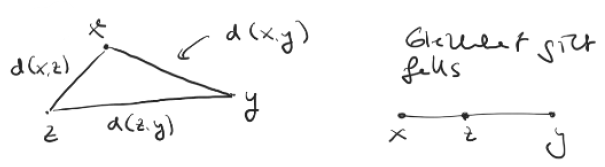
\includegraphics[width=0.8\linewidth]{figures/dreiecksungleichung_visualisierung}
    \label{fig:dreiecksungleichung_visualisierung}
\end{figure}
\begin{definition}\index{$\varepsilon$-Ball}
    Sei \( (X,d) \) ein metrischer Raum. Seien \( x\in X \), \( \varepsilon>0 \). Dann nennt man
    \begin{align*}
        \ball{\epsilon}{x}\definedas\Set{y\in X| \distance{x}{y}<\varepsilon}
    \end{align*}
    den (offenen) \( \varepsilon \)-Ball um \( x \).
\end{definition}
\begin{beispiele*}
    \begin{enumerate}
        \item \( \ball{\varepsilon}{x}=\ointerval{x-\varepsilon}{x+\varepsilon} \).
        \item \( \ball{\varepsilon}{x}=\begin{cases}
            x & \varepsilon\leq 1 \\
            X & \varepsilon>1
        \end{cases}
         \)
         
        \item \( \ball{\varepsilon}{x}= \) \raisebox{-2em}{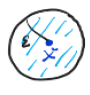
\includegraphics[width=0.1\linewidth]{figures/offener_ball_r_n}}
        
    \end{enumerate}
\end{beispiele*}
\begin{satz}\label{metrische_topologie}
    Sei \( (X,d) \) ein metrischer Raum. Dann wird durch
    \begin{align*}
        \mathcal{T}_d\definedas \Set{U\subset X|\forall x\in U\logicspace\exists\varepsilon>0\logicspace\text{\sd}\logicspace \ball{\varepsilon}{x}\subset U}
    \end{align*}
    eine Topologie definiert.
\end{satz}
\begin{proof}
    Als Hausaufgabe.    
\end{proof}
\begin{bemerkungen}
    \begin{enumerate}
        \item \ref{standard-topologie} ist ein Spezialfall dieser Aussage
        \item Die \enquote{offenen} \( \varepsilon \)-Bälle sind tatsächlich offen: Zu \( y\in \ball{\varepsilon}{x} \) wähl \( \tilde{\varepsilon}\definedas \varepsilon-\distance{x}{y}>0 \).
        \begin{figure}[H]
            \centering
            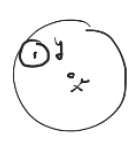
\includegraphics[width=0.3\linewidth]{figures/offene_baelle_sind_offen}
            \label{fig:offene_baelle_sind_offen}
        \end{figure}
        Dann ist \( \ball{\tilde{\varepsilon}}{y}=\Set{z|\distance{y}{z}<\tilde{\varepsilon}} \subset \ball{\varepsilon}{x}\). Denn für alle \( z\in \ball{\tilde{\varepsilon}}{y} \) ist
        \begin{align*}
            \distance{x}{z}\begin{aligned}[t] 
                &\leq \distance{x}{y}+\distance{y}{z}<\distance{x}{y}+\tilde{\varepsilon}\\
                &=\distance{x}{y}+\varepsilon-\distance{x}{y}=\varepsilon
            \end{aligned}
        \end{align*}
        
        \item Bezüglich der diskreten Metrik ist \emph{jede} Teilmenge offen.
        \item Die Klumpentopologie wird nicht von einer Metrik erzeugt (wenn \( X \) mehr als \( 1 \) Element enthält).
        \begin{proof}
            Seien \( x,y\in X \), \( x\neq y \). Angenommen \texists Metrik \( d \).
            \begin{align*}
                \implies &\distance{x}{y}\neq 0\implies \distance{x}{y}=c>0\\
                \implies &\ball{c}{x}\text{ ist offen.}\\
                \underset{\text{\scshape{VOR}}}{\implies} &\ball{c}{x}=\emptyset \text{ oder } =X\\
                \implies &\ball{c}{x}=X
            \end{align*}
            \contra, da \( y\notin \ball{c}{x} \).
            
        \end{proof}
        
        \item \label{metrischer_raum_ist_hausdorffsch} Ein metrischer Raum ist hausdorffsch. \tto HA\@.
        
    \end{enumerate}
\end{bemerkungen}
Wir formulieren nun Konvergenz und Stetigkeit für metrische Räume:
\begin{bemerkungen}
    Sei \( (X,d) \) metrischer Raum.
    \begin{enumerate}
        \item[\thref{umgebung_in_topologischen_raeumen}]\label{umgebung_in_metrischen_raeumen} \( V\subset X \) heißt Umgebung von \( x\in X \), falls es \( \varepsilon >0 \) gibt \sd \( \ball{\varepsilon}{x}\subset U \).
        \item[\thref{konvergenz_in_topologischen_raeumen}]\label{konvergenz_in_metrischen_raeumen} \( (x_n)_n \) konvergiert mit Grenzwert \( x \), falls es zu jedem \( \varepsilon>0 \) ein \( N\in \naturals \) gibt \sd \( x_n\in \ball{\varepsilon}{x}\logicspace\forall n\geq N \).
        \item[\thref{stetigkeit_in_topologischen_raeumen}]\label{stetigkeit_in_metrischen_raeumen} Sei \( (Y,\tilde{d}) \) weiterer metrischer Raum, \( f\maps X \to Y \) eine Abbildung. Dann ist \( f \) stetig \( a \) \gdw:
        \begin{align*}
            \forall\varepsilon>0\logicspace\exists \delta>0\logicspace\text{\sd} f(\ball{\delta}{a})\subset B_\varepsilon(f(a)).
        \end{align*}
    \end{enumerate}
\end{bemerkungen}
\begin{bemerkungen*}
    \begin{enumerate}
        \item \ref{stetigkeit_in_metrischen_raeumen} ist das \( \varepsilon \)-\( \delta \)-Kriterium.
        \item Die Einschränkung auf \( \varepsilon \)-Bälle in \ref{konvergenz_in_metrischen_raeumen} und \ref{stetigkeit_in_metrischen_raeumen} (statt allgemeiner Umgebungen) ist keine echte Einschränkung: Gilt etwas für all Umgebungen, so speziell auch für \( \varepsilon \)-Bälle.
        
        Und gilt eine Inklusion für alle \( \varepsilon \)-Bälle (etwa \( x_n\in \ball{\varepsilon}{x}\logicspace\forall n \geq N(\varepsilon) \)), so auch für beliebige Umgebungen \( U \) von \( x \), da es immer einen \( \varepsilon \)-Ball \( \ball{\varepsilon}{x} \) gibt, der ganz in \( U \) enthalten ist.
    \end{enumerate}
\end{bemerkungen*}
\begin{beispiele}
    \begin{enumerate}
        \item \( \reals^m \) mit der Euklidischen Metrik. \( (x_n)_{n\geq 1} \) Folge in \( \reals^m \), also \( n\mapsto x_n=(x_n^{(1)},\ldots, x_n^{(m)})\in \reals^m \).
        \item \( x_n=\p*{ \frac{1}{n}\Cos+{n},\frac{1}{n}\Sin+{n},a,\ldots,a } \)
        \begin{behauptung*}
            \( x_n\goesto (0,0,a,\ldots,a)\defines x \).
        \end{behauptung*}
        \begin{proof}
            Sei \( \varepsilon>0 \). Es gilt
            \begin{align*}
                &\distance{x_n}{x}^2 \begin{aligned}[t] 
                    &=\sum\limits_{i=1}^{m} (x_n^{(i)}-x^{(i)})^2\\
                    &=\p*{ \frac{1}{n}\Cos+{n}-0 }^2+\p*{ \frac{1}{n}\Sin+{n}-0 }^2+(a-a)^2+\cdots +(a-a)^2\\
                    &=\frac{1}{n^2}(\Cos+{n}^2+\Sin+{n}^2)=\frac{1}{n^2}
                \end{aligned}\\
                \implies &\distance{x_n}{x}=\frac{1}{n}\\
                \implies &\distance{x_n}{x}<\varepsilon\logicspace\forall n\geq N\text{ mit } N>\frac{1}{\varepsilon}\\
                \implies &x_n \in \ball{\varepsilon}{x} \logicspace\forall n \geq N.
            \end{align*}            
        \end{proof}
        
        \item \( X=\stetigefunktionen(\interval{a}{b}) \), \( \distance{f}{g}\definedas \supnorm{f-g} \) mit \( \supnorm{f-g}=\sup_{x\in \interval{a}{b}}\abs{f(x)-g(x)} \).
        \begin{enumerate}[label=\textbf{\arabic*. Beh}]
            \item \( d \) ist eine Metrik auf \( X \).
            \begin{proof}
                \begin{proofdescription}
                    
                    \item[\ref{metrik:nicht_ausgeartet}:]
                    \begin{align*}
                        &\sup_{x\in \interval{a}{b}}\abs{f(x)-g(x)}=0\\
                        \iff &\abs{f(x)-g(x)}=0\logicspace\forall x\\
                        \iff f(x)=g(x)\logicspace\forall x.
                    \end{align*} 
                    
                    \item[\ref{metrik:symmetrisch}:]
                    \begin{align*}
                        &\abs{f(x)-g(x)}=\abs{g(x)-f(x)}\logicspace\forall x\\
                        \implies &\distance{f}{g}=\distance{g}{f}.
                    \end{align*} 
                    \item[\ref{metrik:dreiecksungleichung}:]
                     \begin{align*}
                         &\abs{f(x)-g(x)}\begin{aligned}[t] 
                             &=\abs{f(x)-h(x)+h(x)-g(x)}\\
                             &\explain{\triangle-\text{\Ungl für \( \abs{\cdot} \) auf \( \reals \)}}{\leq} \abs{f(x)-h(x)}+\abs{h(x)-g(x)}
                         \end{aligned}\\
                         \implies& \triangle\text{-\Ungl für \( d \)}.
                     \end{align*}
                \end{proofdescription}
                
            \end{proof}
            
            \item \( (f_n)_n\subset \stetigefunktionen(\interval{0}{1}) \), \( f_n(x)=x^n \), konvergiert nicht (\vgl \diffcourse{1}).
            \begin{proof}
                Wir wissen aus der \diffcourse{1}, dass wenn Konvergenz vorliegt, der Grenzwert gleich dem punktweisen Grenzwert ist. Dieser ist
                \begin{align*}
                    f(x)=\begin{cases}
                        1 & x=1\\
                        0 & \text{sonst}
                    \end{cases}.
                \end{align*}
                Aber
                \begin{align*}
                    \sup_{x\in \interval{0}{1}}\abs{f_n(x)-f(x)}=\sup_{x\in \rinterval{0}{1}}\abs{x^n}=1.
                \end{align*}
            \end{proof}
            
        \end{enumerate}
        \item \( X=\stetigefunktionen(\interval{0}{1}) \), \( \distance{f}{g}=\Integrate{\abs{f(x)-g(x)}}{x,0,1} \).
        \begin{enumerate}[label=\textbf{\arabic*. Beh}]
            
            \item \( d \) ist eine Metrik auf \( \stetigefunktionen(\interval{0}{1}) \).
            \begin{proof}
                HA\@.
            \end{proof}
            
            \item \( (f_n)_n\subset \stetigefunktionen(\interval{0}{1}) \), \( f_n(x)=x^n \) konvergiert, und zwar gegen \( f(x)=0\logicspace\forall x \).
            \begin{proof}
                \begin{align*}
                    &\Integrate{\abs*{f_n(x)-0}}{x,0,1}%=\Integrate{x^n}{x,0,1}=\frac{1}{n+1}\evaluatebetween{x^{n+1}}{x}{0}{1}=\frac{1}{n+1}\\ 
                    \implies &\distance{f_n}{f}=\frac{1}{n+1}<\varepsilon\logicspace\forall n\geq N \text{ mit } N \geq \frac{1}{\varepsilon}.
                \end{align*}
            \end{proof}
            
        \end{enumerate}
        
    \end{enumerate}
\end{beispiele}
 sie